\documentclass[]{article}
\usepackage{caption}
\usepackage{tocloft}
\usepackage{amssymb,amsmath}
\usepackage{ifxetex,ifluatex}
\usepackage{fixltx2e} % provides \textsubscript

\usepackage{longtable}
\usepackage{graphicx}
\usepackage{tikz}

% This function draws a matrix.
\newcommand{\mat}[2]{% cols, rows
\vcenter{\hbox{ %Vertical alignment
\begin{tikzpicture}[scale=0.5, align=center]
\filldraw[step=1,black] (0.0, 0.0) grid (#1, #2);
\end{tikzpicture}
}}}

% This function draws a matrix with a label above it.
\newcommand{\labmat}[3]{% cols, rows, label
\stackrel{#3}{
\vcenter{\hbox{ %Vertical alignment
\begin{tikzpicture}[scale=0.5, align=center]
\filldraw[step=1,black] (0.0, 0.0) grid (#1, #2);
\end{tikzpicture}
}}}}

% This function allows for shading
% cols, rows, cols_shade_start, rows_shade_start, cols_shade_end, rows_shade_end, label
\newcommand{\colormat}[7]{
\stackrel{#7}{
\vcenter{\hbox{ %Vertical alignment
\begin{tikzpicture}[scale=0.5, align=center]
\filldraw[step=1] (0.0, 0.0) grid (#1, #2);
\filldraw[shift={(#4, #3)}, fill=gray] (0, 0) rectangle (#6, #5);
\end{tikzpicture}
}}}}


% nord
\definecolor{blue1}{HTML}{1d71d1}
\definecolor{blue2}{HTML}{0f335c}
\definecolor{blue3}{HTML}{106cc9}
\definecolor{blue4}{HTML}{2f6194}
\definecolor{blue5}{HTML}{2b72bd}
\definecolor{blue6}{HTML}{5894d1}
\definecolor{blue7}{HTML}{61a3ff}
\definecolor{blue8}{HTML}{1750bf}
\definecolor{blue9}{HTML}{d9ebff}
\definecolor{blue10}{HTML}{abd3ff}
\definecolor{blue11}{HTML}{85c0ff}

%

\newcommand{\evenmat}[1]{
\stackrel{#1}{
\vcenter{\hbox{ %Vertical alignment
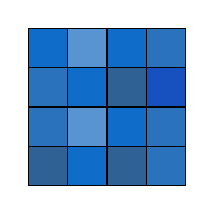
\begin{tikzpicture}[scale=0.5, align=center]
\filldraw[step=1] (0.0, 0.0) grid (4,4);

\filldraw[shift={(0,0)}, fill=blue4] (0, 0) rectangle (1,1);
\filldraw[shift={(1,0)}, fill=blue3] (0, 0) rectangle (1,1);
\filldraw[shift={(2,0)}, fill=blue4] (0, 0) rectangle (1,1);
\filldraw[shift={(3,0)}, fill=blue5] (0, 0) rectangle (1,1);


\filldraw[shift={(0,1)}, fill=blue5] (0, 0) rectangle (1,1);
\filldraw[shift={(1,1)}, fill=blue6] (0, 0) rectangle (1,1);
\filldraw[shift={(2,1)}, fill=blue3] (0, 0) rectangle (1,1);
\filldraw[shift={(3,1)}, fill=blue5] (0, 0) rectangle (1,1);


\filldraw[shift={(0,2)}, fill=blue5] (0, 0) rectangle (1,1);
\filldraw[shift={(1,2)}, fill=blue3] (0, 0) rectangle (1,1);
\filldraw[shift={(2,2)}, fill=blue4] (0, 0) rectangle (1,1);
\filldraw[shift={(3,2)}, fill=blue8] (0, 0) rectangle (1,1);


\filldraw[shift={(0,3)}, fill=blue3] (0, 0) rectangle (1,1);
\filldraw[shift={(1,3)}, fill=blue6] (0, 0) rectangle (1,1);
\filldraw[shift={(2,3)}, fill=blue3] (0, 0) rectangle (1,1);
\filldraw[shift={(3,3)}, fill=blue5] (0, 0) rectangle (1,1);
\end{tikzpicture}
}}}}


\newcommand{\unevenmat}[1]{
\stackrel{#1}{
\vcenter{\hbox{ %Vertical alignment
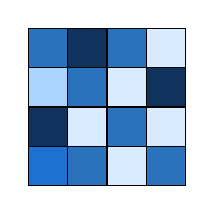
\begin{tikzpicture}[scale=0.5, align=center]
\filldraw[step=1] (0.0, 0.0) grid (4,4);

\filldraw[shift={(0,0)}, fill=blue1] (0, 0) rectangle (1,1);
\filldraw[shift={(1,0)}, fill=blue5] (0, 0) rectangle (1,1);
\filldraw[shift={(2,0)}, fill=blue9] (0, 0) rectangle (1,1);
\filldraw[shift={(3,0)}, fill=blue5] (0, 0) rectangle (1,1);


\filldraw[shift={(0,1)}, fill=blue2] (0, 0) rectangle (1,1);
\filldraw[shift={(1,1)}, fill=blue9] (0, 0) rectangle (1,1);
\filldraw[shift={(2,1)}, fill=blue5] (0, 0) rectangle (1,1);
\filldraw[shift={(3,1)}, fill=blue9] (0, 0) rectangle (1,1);


\filldraw[shift={(0,2)}, fill=blue10] (0, 0) rectangle (1,1);
\filldraw[shift={(1,2)}, fill=blue5] (0, 0) rectangle (1,1);
\filldraw[shift={(2,2)}, fill=blue9] (0, 0) rectangle (1,1);
\filldraw[shift={(3,2)}, fill=blue2] (0, 0) rectangle (1,1);


\filldraw[shift={(0,3)}, fill=blue5] (0, 0) rectangle (1,1);
\filldraw[shift={(1,3)}, fill=blue2] (0, 0) rectangle (1,1);
\filldraw[shift={(2,3)}, fill=blue5] (0, 0) rectangle (1,1);
\filldraw[shift={(3,3)}, fill=blue9] (0, 0) rectangle (1,1);
\end{tikzpicture}
}}}}


\newcommand{\unevenvec}[1]{
\stackrel{#1}{
\vcenter{\hbox{ %Vertical alignment
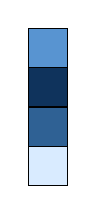
\begin{tikzpicture}[scale=0.5, align=center]
\filldraw[step=1] (0.0, 0.0) grid (1,4);
\filldraw[shift={(0,0)}, fill=blue9] (0, 0) rectangle (1,1);
\filldraw[shift={(0,1)}, fill=blue4] (0, 0) rectangle (1,1);
\filldraw[shift={(0,2)}, fill=blue2] (0, 0) rectangle (1,1);
\filldraw[shift={(0,3)}, fill=blue6] (0, 0) rectangle (1,1);
\end{tikzpicture}
}}}}

\newcommand{\evenvec}[1]{
\stackrel{#1}{
\vcenter{\hbox{ %Vertical alignment
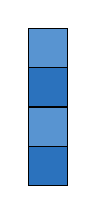
\begin{tikzpicture}[scale=0.5, align=center]
\filldraw[step=1] (0.0, 0.0) grid (1,4);
\filldraw[shift={(0,0)}, fill=blue5] (0, 0) rectangle (1,1);
\filldraw[shift={(0,1)}, fill=blue6] (0, 0) rectangle (1,1);
\filldraw[shift={(0,2)}, fill=blue5] (0, 0) rectangle (1,1);
\filldraw[shift={(0,3)}, fill=blue6] (0, 0) rectangle (1,1);
\end{tikzpicture}
}}}}


\newcommand{\inputvec}[1]{
\stackrel{#1}{
\vcenter{\hbox{ %Vertical alignment
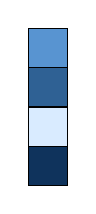
\begin{tikzpicture}[scale=0.5, align=center]
\filldraw[step=1] (0.0, 0.0) grid (1,4);
\filldraw[shift={(0,0)}, fill=blue2] (0, 0) rectangle (1,1);
\filldraw[shift={(0,1)}, fill=blue9] (0, 0) rectangle (1,1);
\filldraw[shift={(0,2)}, fill=blue4] (0, 0) rectangle (1,1);
\filldraw[shift={(0,3)}, fill=blue6] (0, 0) rectangle (1,1);
\end{tikzpicture}
}}}}

\newcommand{\outputvectwo}[1]{
\stackrel{#1}{
\vcenter{\hbox{ %Vertical alignment
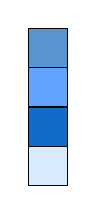
\begin{tikzpicture}[scale=0.5, align=center]
\filldraw[step=1] (0.0, 0.0) grid (1,4);
\filldraw[shift={(0,0)}, fill=blue9] (0, 0) rectangle (1,1);
\filldraw[shift={(0,1)}, fill=blue3] (0, 0) rectangle (1,1);
\filldraw[shift={(0,2)}, fill=blue7] (0, 0) rectangle (1,1);
\filldraw[shift={(0,3)}, fill=blue6] (0, 0) rectangle (1,1);
\end{tikzpicture}
}}}}


\newcommand{\popA}[2]{
\stackrel{#1}{
\vcenter{\hbox{ %Vertical alignment
\begin{tikzpicture}[scale=#2, align=center]
\filldraw[step=1] (0.0, 0.0) grid (1,1);
\filldraw[shift={(0,0)}, fill=blue6] (0, 0) rectangle (1,1);
\end{tikzpicture}
}}}}

\newcommand{\popB}[2]{
\stackrel{#1}{
\vcenter{\hbox{ %Vertical alignment
\begin{tikzpicture}[scale=#2, align=center]
\filldraw[step=1] (0.0, 0.0) grid (1,1);
\filldraw[shift={(0,0)}, fill=blue4] (0, 0) rectangle (1,1);
\end{tikzpicture}
}}}}

\newcommand{\popC}[2]{
\stackrel{#1}{
\vcenter{\hbox{ %Vertical alignment
\begin{tikzpicture}[scale=#2, align=center]
\filldraw[step=1] (0.0, 0.0) grid (1,1);
\filldraw[shift={(0,0)}, fill=blue9] (0, 0) rectangle (1,1);
\end{tikzpicture}
}}}}

\newcommand{\popD}[2]{
\stackrel{#1}{
\vcenter{\hbox{ %Vertical alignment
\begin{tikzpicture}[scale=#2, align=center]
\filldraw[step=1] (0.0, 0.0) grid (1,1);
\filldraw[shift={(0,0)}, fill=blue2] (0, 0) rectangle (1,1);
\end{tikzpicture}
}}}}

\usepackage{hyperref}
\hypersetup{breaklinks=true,
bookmarks=true, colorlinks=true, citecolor=blue, urlcolor=blue, linkcolor=magenta}   


\setlength{\parindent}{0pt}
\setlength{\parskip}{6pt plus 2pt minus 1pt}
\setlength{\emergencystretch}{3em}  % prevent overfull lines
\setcounter{secnumdepth}{0}

\usepackage[left=1in,right=1in]{geometry}
\usepackage{float}
\floatplacement{figure}{h}


\setcounter{secnumdepth}{3}
\addtocontents{toc}{\setcounter{tocdepth}{2}}

\usepackage{sectsty}
\usepackage[normalem]{ulem}
\sectionfont{\rmfamily\bfseries\large}
\subsectionfont{\rmfamily\upshape\large}
\subsubsectionfont{\centering\normalsize}

\fontsize 12
\usepackage{hyperref}
\usepackage{lineno}
\linenumbers
\usepackage[font={footnotesize,sf}]{caption}
\usepackage{siunitx}

\usepackage{setspace}
\linespread{1.5}

\hyphenpenalty 10000 % no hyphens!

\raggedbottom

\usepackage{titling}
\pretitle{\Large}
\preauthor{\large}
\predate{\normalsize}
\postdate{}


\usepackage{fancyhdr}
\pagestyle{fancy}
\lhead{  \nouppercase  \leftmark}
\rhead{\thepage}
\cfoot{}

\usepackage{authblk}

\title{When can we approximate dispersal with diffusion in ecological models?  \\}
\author[1,2]{Michael D. Catchen} 
\author[1]{Samuel M. Flaxman}
\affil[1]{\small{Department of Ecology and Evolutionary Biology, University of Colorado at Boulder}}
\affil[2]{\small{Department of Biology, McGill University}}
\date{\today}


\usepackage[square, numbers]{natbib}
\bibliographystyle{unsrtnat}
\begin{document}

\maketitle{}
\begin{abstract}

In ecology, spatial models have long approximated the dispersal of biological entities using diffusion models \cite{hastings_1978, okubo_diffusion_2001}.
We show that approximating dispersal with diffusion only works under some sets of demographic conditions.
We define a model of metapopulation dynamics on spatial graphs. 
We simulate metapopulation dynamics, where local dynamics occur according to variations on 
the Ricker model \cite{melbourne_hastings_2008}, and dispersal occurs either stochastic dispersal and diffusion. 
We show that the dynamics produced by this model under stochastic dispersal differ from those produced by diffusion under certain parameterizations of the model. 
We do this by measuring the synchrony of the dynamics across populations. We show that under some parameterizations, diffusion and stochastic dispersal models produce similarly synchronous dynamics across populations.
We identify two regimes--one where the variability in the abundances is primarily driven by 
the stochasticity of dispersal, and another where the variability in abundance over time is primarily driven by the forces contributing to stochasticity \textit{within} each population.
We show that as the spatial metric becomes more modular, the diffusion approximation approaches stochastic dispersal.

\end{abstract}
\clearpage
\tableofcontents
\clearpage




\clearpage
\section{Introduction}

Human's impact nearly the entirety of planet earth \cite{watson_protect_2018}.
Climate change is exposing all ecosystems to rapidly shifting temperatures \cite{pereira_scenarios_2010}, and land-use change is causing terrestrial habitats to become smaller and patchier \cite{haddad_habitat_2015}. As a result, understanding and predicting the impacts of landscape change on Earth's ecosystems remains a central goal of modern ecological research \cite{fletcher_spatial_2019, fischer_landscape_2007}---both to impede ongoing loss of biodiversity, and to plan sustainable development to mitigate the effects of climate change \cite{albert_applying_2017,baguette_individual_2013}. 
It has widely been shown that the spatial structure of habitat influences the dynamics of the ecological processes that occur in that habitat \cite{haddad_experimental_2017, ricketts_matrix_2001, gilbert_corridors_1998, taylor_connectivity_1993}, and that increased \textit{landscape connectivity} can mitigate the effect of habitat loss on biodiversity. 
\cite{resasco_meta-analysis_2019,
thompson_loss_2017, chisholm_metacommunity_2011}. 

In order to design landscapes that mitigate biodiversity loss and its effects, we need models to understand how landscape connectivity affects the dynamics of ecological processes. In ecology and other fields, spatial processes have long been modeled with \textit{diffusion} \cite{cantrell_spatial_2004, okubo_diffusion_2001, hastings_global_1978}.
Diffusion is often used to model the movement and dispersal of organisms. However, dispersal is inherently a stochastic process, which diffusion approximates with its expected value at each timestep. We show that in the context of metapopulation dynamics, diffusion models can generate highly synchronized dynamics across space where stochastic dispersal does not.

Synchrony of population dynamics is widely observed in real systems \cite{}. It is broadly understood that spatial synchrony is largely driven by covariance in environmental conditions across habitat patches \cite{}. Here, we model each populations local dynamics independently to isolate the effect of migration on causing synchrony---we use the synchrony of population dynamics as a measure of \textit{functional} connectivity \cite{}, meaning that in the context of metapopulation dynamics, movement between populations represents process driving connectivity: abundances shifting due to migration. 

We show that both the modularity of the habitat network (represented by a spatial graph) and the demographic parameters of local population dynamics effect the validity of approximating dispersal with diffusion. We also show that total synchrony is a product of the even-mixing of local demographic stochasticity via dispersal. We do this by presenting a spatial graph model of dispersal, and then simulating metapopulation dynamics by combining a Ricker model of local population dynamics with either diffusion or stochastic dispersal. 
We implement the software to used run these simulations as a Julia package `MetapopulationDynanmics.jl`.

\section{A Model of Metapopulation Dynamics of Spatial Graphs}

Here, we present a model of metapopulation dynamics on spatial graphs, which is implemented in the package `MetapopulationDynamics.jl`. 
The package includes a generative spatial graph model of landscape connectivity, and methods for simulating batch sets of dynamics with arbitrary summary statistics. 

\subsection{Spatial Graph Model of Landscape Connectivity}
Spatial graphs have long been used to model a system of habitat patches
\cite{dale_graphs_2010, minor_graph-theory_2008,
urban_landscape_2001}. 
Here we model a system of populations, represented as a vector of
vertices $\vec{L}$ in a spatial graph $G$, where the edges represent dispersal between populations. In order to define how the edges of this network describe dispersal, we choose to model landscape connectivity as a combination of two different factors: the probability than any individual migrates during its lifetime, $m$, and the conditional distribution over spatial nodes of where an individual goes ($j \in L$), given both that
it migrates $m$ and where it started ($i \in L$), which we call the dispersal potential and denote $$\Phi_{ij} =  P(L_j|L_i, m)$$

The dispersal potential can be modeled several ways. In empirical systems, it can be estimated with resistance surfaces, which provide
relative weights of the difficulty of movement between pairs of cells on a
raster \cite{spear_use_2010}. Here, however, we model
the dispersal potential using isolation-by-distance (IBD), which assumes the relative probability of dispersal $L_i \to L_j$ is inversely
proportional to the distance between them, \(d_{ij}\), and the strength
of this isolation-by-distance relationship, \(\alpha\). For the functional form of the IBD relationship, called the dispersal kernel \cite{grilli_metapopulation_2015, hanski_practical_1994}, we consider an exponential
with decay-strength $\alpha$ and a cutoff value $\epsilon$, 
$$f(d_{ij}, \alpha, \epsilon) =  \begin{cases}
        e^{-\alpha d_{ij}} \quad\quad\quad &\text{if}\quad e^{-\alpha d_{ij}} > \epsilon \ \ \text{and } i \neq j \\   0 &\text{else}
\end{cases}$$

Then, to construct a dispersal potential $\Phi_{ij}$ with a kernel $f(d_{ij}, \alpha)$,  we normalize:

$$\Phi_{ij} = \frac{f(d_{ij}, \alpha, \epsilon)}{\sum_k f(d_{ik},\alpha, \epsilon)}$$

Note that the sum of each row of $\Phi$, forms a probability distribution, i.e. $\sum_j \Phi_{ij} = 1 \ \ \forall i$. In some cases, for a given location $i$,  $f(d_{ij}, \alpha, \epsilon)$ could be $0$ for all $j$, in which case $\Phi_{ii}$ is set to $1$ to enforce this condition. Also note that if $\alpha=0$, the dispersal potential is a uniform distribution over locations. In Figure \ref{fig:mp}, we can see the same set of points plotted spatial graphs plotted representing the same set of populations across differing values of $\alpha$. 


\begin{figure}[H]
    \centering
    \includegraphics[width=15cm]{figs/metapops.png}
    \caption{Caption}
    \label{fig:mp}
\end{figure}

\subsection{Dynamics}

\subsubsection{Local Population Dynamics}

We model local population dynamics using a Poisson Ricker Model. We consider the simplest variation on the model, which only includes demographic stochasticity, however it is straightforward to extend this to other forms of stochasticity \cite{melbourne_extinction_2008}.

At each timestep, the abundance $N_i$ at location $i$ is drawn as

$$N_i(t+1) \sim \text{Poisson}\bigg(N_i(t) \lambda R e^{- \chi N_i(t)}\bigg)$$

where $\chi$ represents the strength of mortality of surviving until adulthood, $R$ is the probability that an adult reproduces ($0.9$ for all results presented here), and where $\lambda$ is the mean number of offspring for each individual that reproduces---yielding three total parameters: $\theta = \{\lambda, R, \chi \}$. 




\subsubsection{Stochastic Dispersal}


To model stochastic dispersal, for each location $i$, the number of migrants leaving that location is drawn 

$$n_{i} \sim \text{Binomial}(N_i, m)$$

and for every migrating indiviudal $\in \{1, \dots, n_i\}$ we draw where that individual goes directly from the distribution $\Phi_i$.

\subsection{Measuring Synchrony}
In ecology, the crosscorrelation function, \(CC\), has long been used as a measure of synchronous dynamics \cite{liebhold_spatial_2004}. Here, with a subdivided
population, we consider the mean crosscorrelation compared across all populations, $${PCC}=\frac{1}{n^2}\sum_{i,j} CC(A_i,A_j)$$  

\subsubsection{Diffusion Dispersal}


To model dispersal using diffusion, we incorporate the Ricker Model into a reaction-diffusion model. If the probability that an individual migrates before reproducing is $m$, then we can define a diffusion matrix $D$ as 

$$D_{ij} = \begin{cases} \Phi_{ij}m \quad\quad\quad &\ i \neq j \\ 1-m  & i=j \end{cases}$$

where $D_{ij}$ is the probability that a unit biomass that is born in $i$ reproduces in $j$.

Then, the spatial dynamics of this model are described by the mapping $$N_i(t+1) = \sum_j D_{ji} N_j(t)$$


\begin{equation}
  \unevenvec{N(t+1)}  = \begin{bmatrix} \ \  \unevenmat{D^T} \boldsymbol{\cdot} \inputvec{N(t)} \ \ \vspace{1em} \end{bmatrix} 
\end{equation}


which can be combined into the local Ricker model from above as reaction-diffusion model by computing diffusion before each round of local dynamics.

$$N_i(t+1) \sim \text{Poisson}\bigg( \lambda R e^{-\chi \big(\sum_j D_{ji} N_j(t)\big)} \cdot \sum_j D_{ji} N_j(t) \bigg)$$


\begin{equation}
 \outputvectwo{N(t+1)} = \text{RickerModel} \Bigg ( 
        \begin{bmatrix}\unevenmat{D^T} \boldsymbol{\cdot} \inputvec{N(t)} \vspace{0.3em} \end{bmatrix}
\Bigg)
\end{equation}



\subsection{Measuring Synchrony}

In ecology and other fields, the crosscorrelation function, \(CC\), has long been used as a measure of synchronous dynamics \cite{liebold_spatial_2004}. Here, with a subdivided
population, we consider the mean crosscorrelation compared across all pairs of populations, which we call the Pairwise Crosscorrelation and denote $PCC$. $${PCC}=\frac{1}{n(n-1)}\sum_{i > j} CC(A_i,A_j)$$ 


\subsection{Model Lifecycle}

\begin{figure}[H]
    \centering
    \includegraphics[width=15cm]{figs/conceptual.png}
    \caption{Caption}
    \label{fig:lifecycle}
\end{figure}



\section{Results}

\subsection{Synchrony across a migration gradient}


\begin{figure}[H]
    \centering
    \includegraphics[width=15cm]{figs/migr_grad_over_lambda.png}
    \caption{Caption}
    \label{fig:mig_grad}
\end{figure}

\begin{figure}[H]
    \centering
    \includegraphics[width=15cm]{figs/lambda_and_alpha.png}
    \caption{Caption}
    \label{fig:mig_grad}
\end{figure}


\subsection{The two regimes of stochasticity}


\begin{figure}[H]
    \centering
    \includegraphics[width=8cm]{figs/vary_alpha.png}
        \includegraphics[width=8cm]{figs/vary_epsilon.png}    
    \caption{Caption}
    \label{fig:mig_grad}
\end{figure}


\begin{figure}[H]
    \centering
    \includegraphics[width=15cm]{figs/abundance_v_alpha.png}
    \caption{Caption}
    \label{fig:mig_grad}
\end{figure}


\subsection{Even-mixing causes synchronized dynamics}


\begin{figure}[H]
    \centering
    \includegraphics[width=15cm]{figs/even_mixing_annotated.png}
    \caption{Caption}
    \label{fig:mig_grad}
\end{figure}


\section{Discussion}

\clearpage
{
\footnotesize
\bibliography{references}
}

\section{Supplementary Figures}

\begin{figure}[H]
    \centering
    \includegraphics[width=15cm]{figs/vary_npops.png}
 
    \caption{Caption}
    \label{fig:mig_grad}
\end{figure}

\begin{figure}[H]
    \centering
    \includegraphics[width=15cm]{figs/num_pops_facet.png}
    \caption{Caption}
    \label{fig:mig_grad}
\end{figure}

\begin{figure}[H]
    \centering
    \includegraphics[width=15cm]{figs/abundance_num_pops.png}
 
    \caption{Caption}
    \label{fig:mig_grad}
\end{figure}




\end{document}
